\section{字典排列法}

\title[第2讲\quad 字典排列法]{第2讲\quad 字典排列法} 
\author{}
\date{}
\begin{frame}
    \titlepage
\end{frame}

\begin{frame}
    \frametitle{课前测}
    \textit{用一块长8分米,宽4分米的长方形纸板与两块边长4分米的正方形纸板拼成一个正方形.拼成的正方形的周长是多少分米?}

    \textit{A.12\\ B.24\\ C.32\\ D.40}
\end{frame}

\begin{frame}
    \frametitle{课前测}
    \begin{figure}[H] 
        \centering
        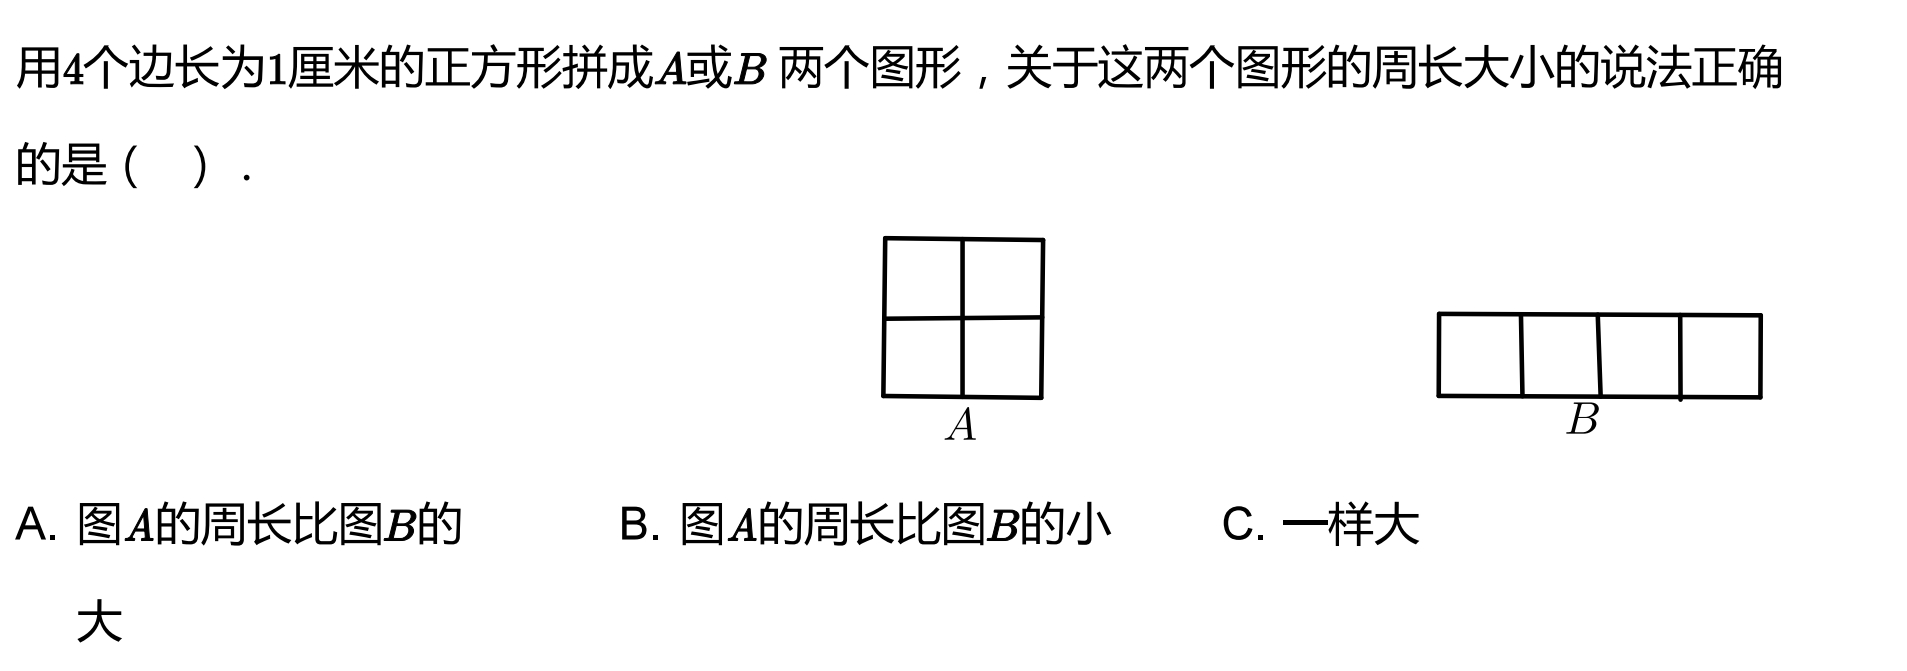
\includegraphics[width=1\textwidth]{./pics/Chapter_2/keqian2.png}
    \end{figure}
\end{frame}

\begin{frame}
    \frametitle{课前测}
    \begin{figure}[H] 
        \centering
        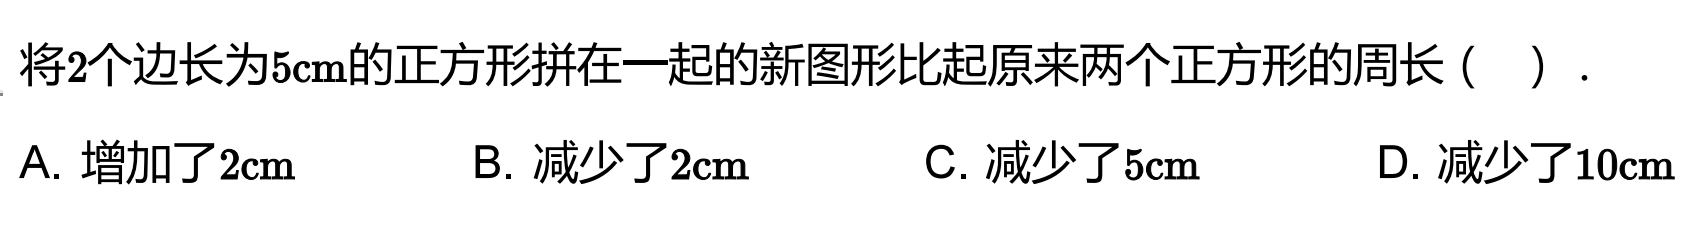
\includegraphics[width=1\textwidth]{./pics/Chapter_2/keqian3.png}
    \end{figure}
\end{frame}

\begin{frame}
    \frametitle{知识梳理}
\end{frame}

\begin{frame}
    \frametitle{MISSION 1}
    \textit{同学们,在进行字典排列法时,我们应当如何做到不重不漏呢?}
\end{frame}

\begin{frame}
    \frametitle{探索1}
    \textit{(1)用数字1、2、3可以组成多少个不同的无重复数字的两位数?}
\end{frame}

\begin{frame}
    \frametitle{探索1}
    \textit{(2)用数字1、3、6可以组成多少个不同的无重复数字的三位数?}
\end{frame}

\begin{frame}
    \frametitle{探索2}
    \textit{(1)用数字1、2、3可以组成多少个不同的两位数?}
\end{frame}

\begin{frame}
    \frametitle{探索2}
    \textit{(2)用数字1、3、6可以组成多少个不同的三位数?}
\end{frame}

\begin{frame}
    \frametitle{探索3}
    \textit{用数字1、2、3可以组成多少个不同的无重复数字的自然数?}
\end{frame}

\begin{frame}
    \frametitle{课堂互动1}
    \begin{figure}[H] 
        \centering
        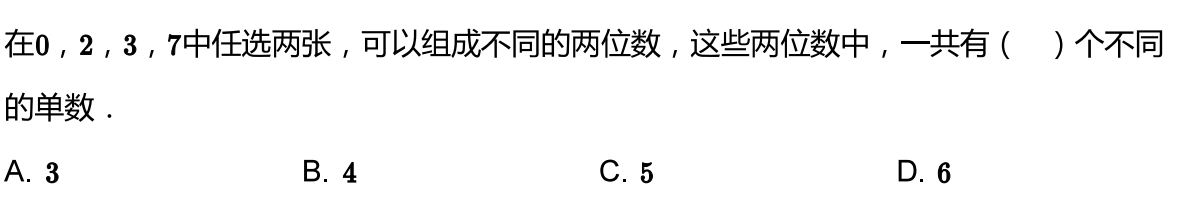
\includegraphics[width=1\textwidth]{./pics/Chapter_2/ketanghudong1.png}
    \end{figure}
\end{frame}

\begin{frame}
    \frametitle{课堂互动2}
    \begin{figure}[H] 
        \centering
        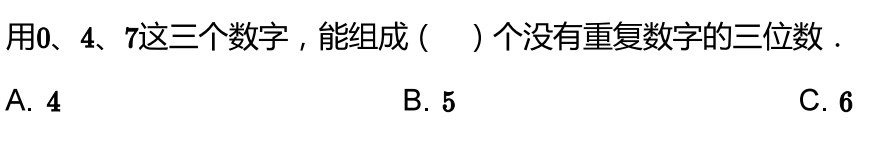
\includegraphics[width=1\textwidth]{./pics/Chapter_2/ketanghudong2.png}
    \end{figure}
\end{frame}

\begin{frame}
    \frametitle{课堂互动3}
    \begin{figure}[H] 
        \centering
        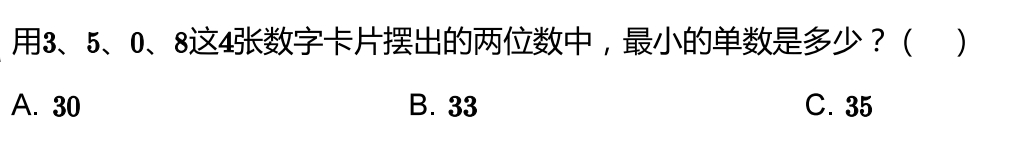
\includegraphics[width=1\textwidth]{./pics/Chapter_2/ketanghudong3.png}
    \end{figure}
\end{frame}

\begin{frame}
    \frametitle{捉虫时刻}
    \textit{艾迪这道题的做法对么?如果不对,请你写一下正确的解法。\\
    用数字1、2能组成多少个不同的三位数 ?\\
    由于要组成三位数,因此有一个数字要重复.\\
    一一列举:112、121、211、221、212、122,共有6个.}
\end{frame}

\begin{frame}
    \frametitle{MISSION 2}
    \textit{在无序问题中,我们应当如何进行枚举?}
\end{frame}

\begin{frame}
    \frametitle{探索4}
    \textit{艾迪与薇儿做游戏,在分别标有1到10的10个完全一样的小球中,艾迪任意取出2个小球(不计取出顺序),由薇儿计算两球所标的数之和,若和大于10,则薇儿获胜.那么能使薇儿获胜的小球取法共有多少种?}
\end{frame}

\begin{frame}
    \frametitle{探索5}
    \textit{艾迪去儿童餐厅买15元特惠套餐,他有若干张1元、2元、5元的纸币,但是购买特惠套餐的条件是必须找出一共有多少种不同的付钱方法(要求每种纸币都有),眼看优惠时间就要截止了,同学们你能帮助艾迪顺利买到优惠套餐吗 ?}
\end{frame}

\begin{frame}
    \frametitle{探索6}
    \textit{在某地有四种不同面值的硬币,如图所示,假若你恰有这四种硬币各1枚。问:共能组成多少种不同的钱数?}
    \begin{figure}[H] 
        \centering
        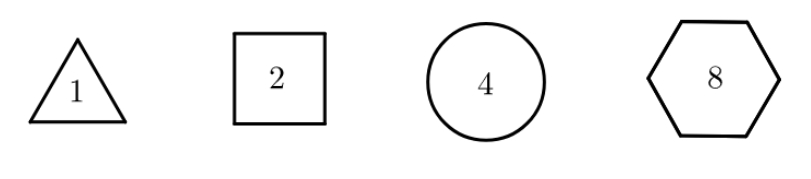
\includegraphics[width=0.5\textwidth]{./pics/Chapter_2/tansuo6.png}
    \end{figure}
\end{frame}

\begin{frame}
    \frametitle{补充1}
    \textit{薇儿收集到四种不同的面值的硬币各1枚,如图所示,一共可以组成多少种不同的钱数?}
    \begin{figure}[H] 
        \centering
        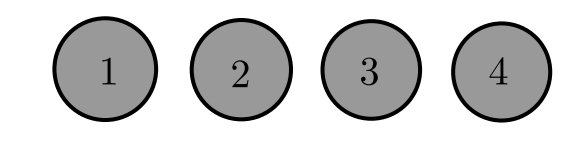
\includegraphics[width=0.3\textwidth]{./pics/Chapter_2/buchong1_1.png}
    \end{figure}
\end{frame}

\begin{frame}
    \frametitle{补充1}
    \textit{艾迪收到三种不同面值的硬币,如图所示,假若你恰好有以下四枚硬币.问共能组成多少种不同的钱数?}
    \begin{figure}[H] 
        \centering
        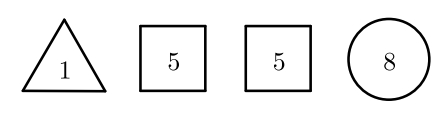
\includegraphics[width=0.3\textwidth]{./pics/Chapter_2/buchong1_2.png}
    \end{figure}
\end{frame}


\begin{frame}
    \frametitle{补充1}
    \textit{用四种不同的硬币各1枚,如图所示,两两一组,一共可以组成多少种不同的钱数?}
    \begin{figure}[H] 
        \centering
        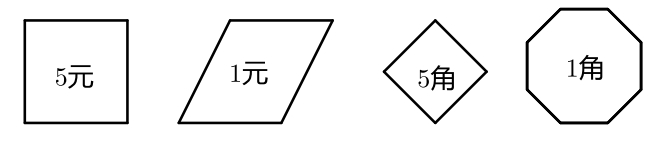
\includegraphics[width=0.3\textwidth]{./pics/Chapter_2/buchong1_3.png}
    \end{figure}
\end{frame}

\begin{frame}
    \frametitle{探索7}
    \textit{博士给艾迪与薇儿上课,课上介绍了``拐弯''的概念.\\
    博士:``对于一行数,如果有三个数abc依次排一起,且a >b,c>b或者a <b,c<b,我们就称它发生了一次拐弯''\\
    艾迪:``我懂了,比如4321没有拐弯,像1243就发生了一次拐弯''\\
    薇儿:``没错,再比如1324就发生了两次拐弯.''\\
    博士:``非常棒!看来你们都掌握得非常扎实了,现在我要考考你们了,如果我们将1,2,3,4排成一行,则能使这行数刚好发生两次拐弯的排列方法共有多少种?''}
\end{frame}

\begin{frame}
    \frametitle{探索8}
    \textit{一次,齐王与田忌赛马,每人各有等级不同的4匹马,这8匹马按照从快到慢的排序分别是齐王的一等马,田忌的一等马,齐王的二等马,田忌的二等马,齐王的三等马,田忌的三等马,齐王的四等马,田忌的四等马.田忌已经提前知道齐王本次赛马的出场顺序是一等、二等、三等、四等,他可以安排种不同的出场顺序,才能保证自己至少战平齐王呢?同学们,你们能帮田忌找出所有可能的决策吗 ?}
\end{frame}

\begin{frame}
    \frametitle{补充2}
    \textit{加加与减减做游戏,两人轮流在一张白纸上写出一个数字,组成一个多位数的前2位,而这个多位数从第三个数字开始,每个数字都恰好是它前面两个数字之和,直至不能再写为止.例如加加减减写了1和4,那么这个多位数就是1459,则这类多位数共有多少个?}
\end{frame}

\begin{frame}
    \frametitle{补充2}
    \textit{如果一个数的各位数字从左到右构成等差数串,我们就称这个数为“跳跃数”,例如:1358642均是“跳跃数”,153就不是“跳跃数”,那么一共有多少个三位“跳跃数”?}
\end{frame}

\begin{frame}
    \frametitle{补充2}
    \begin{figure}[H] 
        \centering
        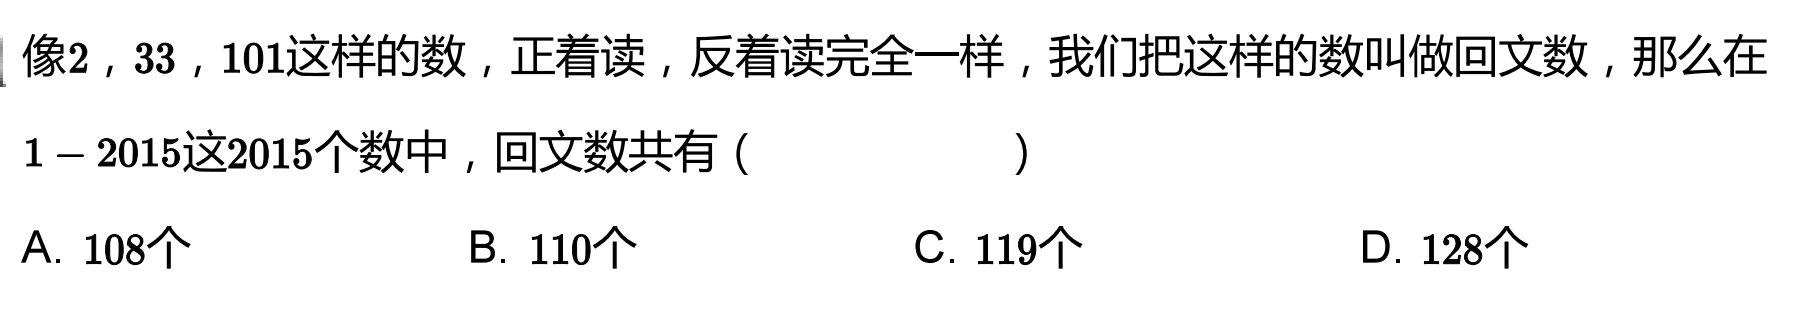
\includegraphics[width=1\textwidth]{./pics/Chapter_2/buchong2_3.png}
    \end{figure}
\end{frame}